\documentclass{beamer}
\usepackage[utf8]{inputenc}
\usepackage[frenchb]{babel}
\usepackage{tikz}
%\usepackage{subfigure}
%\usepackage[scriptsize]{caption}
\usepackage{multicol}
\renewcommand*{\figurename}{}
\usetikzlibrary{shapes,positioning,snakes,calc}
\usetheme{Darmstadt}
\usepackage{graphicx}

% \setbeamercolor{alerted text}{fg=blue}

\title{FMIN327 Cognition individuelle et collective\\ Protocoles artificiels entre agents naturels}
\author{DUPÉRON Georges \and\\ BONAVERO Yoann}
\institute{Université Montpellier II, Département informatique  \\ Master 2 IFPRU \\ Sous la direction de Monsieur Jacques Ferber}
\date{Jeudi, 3 novembre 2011}

\defbeamertemplate*{footline}{shadow theme}
{%
  \leavevmode%
  \hbox{\begin{beamercolorbox}[wd=.5\paperwidth,ht=2.5ex,dp=1.125ex,leftskip=.3cm plus1fil,rightskip=.3cm]{author in head/foot}%
    \usebeamerfont{author in head/foot}\insertframenumber\,/\,\inserttotalframenumber%\hfill\url{http://www.pticlic.fr/}
  \end{beamercolorbox}%
  \begin{beamercolorbox}[wd=.5\paperwidth,ht=2.5ex,dp=1.125ex,leftskip=.3cm,rightskip=.3cm plus1fil]{title in head/foot}%
    \usebeamerfont{title in head/foot}\insertshorttitle%
  \end{beamercolorbox}}%
  \vskip0pt%
}

\AtBeginSection[] { 
  \begin{frame}[plain] 
    \frametitle{Plan} 
    \tableofcontents[currentsection] 
  \end{frame} 
  \addtocounter{framenumber}{-1} 
}

\begin{document}
\renewcommand*{\figurename}{}

\begin{frame}
  \titlepage
\end{frame}

\section{Introduction}

\begin{frame}
  \begin{beamercolorbox}
    Pour se comprendre, il faut des concepts et un mécanisme d'échange communs.
  \end{beamercolorbox}
  \begin{figure}
    \centering
    \begin{tikzpicture}[scale=0.8,every node/.style={transform shape}]
      \begin{scope}
        \node[draw,rectangle,minimum width=3cm,minimum height=2cm,anchor=south west] (ra) at (0,0) {};
        \path[fill=black!50!white](0.7cm,0.7cm) circle (0.3cm);
        \path[fill=green!80!black]  (1.5cm,1.3cm) circle (0.3cm);
        \path[fill=orange] (2.3cm,0.7cm) circle (0.3cm);
        \node[draw,fill=green!30!red,rectangle,minimum width=0.3cm,minimum height=0.3cm] (la1) at (ra.15) {};
        \node[draw,fill=green!50!blue,rectangle,minimum width=0.3cm,minimum height=0.3cm] (la2) at (ra.-15) {};
      \end{scope}
      \begin{scope}[xshift=6cm]
        \node[draw,rectangle,minimum width=3cm,minimum height=2cm,anchor=south west] (rb) at (0,0) {};
        \path[fill=red]   (1cm,1cm) circle (0.3cm);
        \path[fill=blue]  (2cm,1cm) circle (0.3cm);
        \node[draw,fill=white!20!blue!70!red,rectangle,minimum width=0.3cm,minimum height=0.3cm] (lb1) at (rb.165) {};
        \node[draw,fill=green!50!blue,rectangle,minimum width=0.3cm,minimum height=0.3cm] (lb2) at (rb.195) {};
      \end{scope}
      \begin{scope}[xshift=3cm,yshift=3cm]
        \node[draw,rectangle,minimum width=3cm,minimum height=2cm,anchor=south west] (rc) at (0,0) {};
        \path[fill=red]   (0.7cm,0.7cm) circle (0.3cm);
        \path[fill=green!80!black] (1.5cm,1.3cm) circle (0.3cm);
        \path[fill=blue]  (2.3cm,0.7cm) circle (0.3cm);
        \node[draw,fill=white!20!blue!70!red,rectangle,minimum width=0.3cm,minimum height=0.3cm] (lc1) at (rc.270) {};
      \end{scope}
      
      \draw[<->, thick] (lb1)--(lc1);
      \only<2->{\draw[<->, thick, dashed, red] (la2)--(lb2);}
      \only<3->{\draw[<->, thick, dashed, red] (la1)--(lc1);}
    \end{tikzpicture}
    \caption{Communication entre trois agents}
  \end{figure}
  % TODO
  % schéma avec groupe, concepts et échanges
  % montrer si on n'a pas de concepts communs
  % si pas de protocoles communs
  % Mettre un ordi dedans.
\end{frame}

% \begin{frame}
% \begin{block}{Définitions}
% \begin{itemize}
% 	\item Protocole artificiel\\
% 	Règles arbitraires qui codifient l'échange entre des agents.\\
% 	Nous étudierons seulement les protocoles artificiels formels.
% 	\item Agent naturel\\
% 	Entité capable d'interagir non crée par l'homme.
% \end{itemize}
% \end{block}
% \end{frame}

% \section{Espéranto}

% \begin{frame}
% \begin{center}
% \huge Espéranto
% \end{center}
% \begin{itemize}
% \item Origine et but.
% \item Une langue dite \emph{construite}
% \item Une langue vivante.
% \end{itemize}
% \end{frame}

% \begin{frame}
% \begin{center}
% \huge Espéranto
% \end{center}
% \begin{itemize}
% \item Une grammaire régulière.
% \\ Exemple eo + fr.
% \item Une langue agglutinante.
% \\ Exemple eo + fr.
% \end{itemize}
% \end{frame}

% \section[Contrats]{Législation et contrats formels}

% \begin{frame}  
%   \begin{itemize}
%   \item Buisness Contract Language (BCL)% GovMil.pdf
%   \item Formalisation des obligations, permissions, pénalités.% en cas de violation des obligations
%   \item Vérification de la consistance.
%   \end{itemize}
% \end{frame}

% \section[Alphabets]{Alphabets et notations}

% \begin{frame}
%   {\Huge Logogrammes}
%   \begin{itemize}
%   \item Alphabet roman
%   \item Alphabet grec
%   \item \dots
%   \end{itemize}
%   % TODO : images
%   \begin{itemize}
%   \item Idéogrammes chinois
%   \item Hiéroglyphes
%   \item \dots
%   \end{itemize}
% \end{frame}

% \begin{frame}
%   {\Huge Le morse}
%   \begin{itemize}
%   \item Invention attribué à Samuel Morse (1791 - 1872)
%   \item Créé en 1835
%   \item Seulement deux types d'impulsion sont nécessaires.
%   \end{itemize}
%   % Ajouter la photo de Samuel Morse.
  
%   % TODO
%   Un exemple Alphabet écrit en morse.
% \end{frame}


% \begin{frame}  
%   \Huge{Le braille}
%   \begin{center}
%   % TODO
%   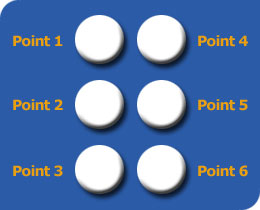
\includegraphics[width=4cm]{./include/cellule_braille.jpg}
%   \end{center}
%   \normalsize \begin{itemize}
%   \item Louis Braille (1809 - 1852)
%   \item Inventé en 1824
%   \item Alphabet en relief
%   \item 64 combinaisons pour tout faire
%   \end{itemize}
% \end{frame}

% \begin{frame}  
%   \Huge Le braille
%   \\ des exemples.
% \end{frame}


% \begin{frame}  
%   { \Huge La langue des signes. }
%   \begin{itemize}
%   \item IBM : programme pour traduire texte vers Langue des signes.
%   \item Facilite la communication avec les malentendants.
%   \item Grammaire assez floue.
%   \item Pas exactement le même vocabulaire que le français.
%   \item Encodage de mots et concepts.
%   \end{itemize}
% \end{frame}

% \begin{frame}  
%   \begin{itemize}
%   \item Vues perspective (ISO...) % TODO
%   \item Vue éclatée
%   \item Notation mathématique
%   \end{itemize}
% % TODO : une vue éclatée
% % TODO : une formule
% \end{frame}

% \section{Conclusion}

% % Graphique avec expressivité vs formel
% % Esperanto : patate 7-10, 4-1
% % Français : patate 7-10, 2-1
% % Braille, morse : point 1, 10
% % Alphabet roman : patate 1, 10-8
% % Alphabets chinois etc. : patate 1-3, 10-6
% % LSF : patate 1-3, 10-6
% % Diagrammes et vues normalisées : point 6, 10
% % BCL (contrats) : point 6, 9

% \begin{frame}
% \end{frame}

\end{document}
